\documentclass[11pt]{article}


\usepackage[letterpaper,margin=1in]{geometry}
\usepackage{graphicx}
\usepackage{hyperref}
\usepackage{amsmath}
\usepackage{amssymb}
\usepackage{bm}
\usepackage{listings}
\usepackage{color}
\usepackage{tikz}
\usepackage{hologo}% or use package holog

\usepackage{empheq}
\usepackage{color}

\usetikzlibrary{decorations.pathmorphing,patterns}

\definecolor{myblue}{rgb}{.92549, .98824, 0.95686}
\newlength\mytemplen
\newsavebox\mytempbox

\makeatletter
\newcommand\mybluebox{%
    \@ifnextchar[%]
       {\@mybluebox}%
       {\@mybluebox[0pt]}}

\def\@mybluebox[#1]{%
    \@ifnextchar[%]
       {\@@mybluebox[#1]}%
       {\@@mybluebox[#1][0pt]}}

\def\@@mybluebox[#1][#2]#3{
    \sbox\mytempbox{#3}%
    \mytemplen\ht\mytempbox
    \advance\mytemplen #1\relax
    \ht\mytempbox\mytemplen
    \mytemplen\dp\mytempbox
    \advance\mytemplen #2\relax
    \dp\mytempbox\mytemplen
    \colorbox{myblue}{\hspace{1em}\usebox{\mytempbox}\hspace{1em}}}

\makeatother

\definecolor{dkgreen}{rgb}{0,0.6,0}
\definecolor{gray}{rgb}{0.5,0.5,0.5}
\definecolor{mauve}{rgb}{0.58,0,0.82}

\lstset{frame=tb,
  language=Python,
  aboveskip=3mm,
  belowskip=3mm,
  showstringspaces=false,
  columns=flexible,
  basicstyle={\small\ttfamily},
  numbers=none,
  numberstyle=\tiny\color{gray},
  keywordstyle=\color{blue},
  commentstyle=\color{dkgreen},
  stringstyle=\color{mauve},
  breaklines=true,
  breakatwhitespace=true,
  tabsize=3
}

\graphicspath{ {./images/} }

\def\changemargin#1#2{\list{}{\rightmargin#2\leftmargin#1}\item[]}
\let\endchangemargin=\endlist 

% define info for title page
\title{AMATH 271 Miniproject 2: \\ Pendulums}
\author{Kamalesh Reddy Paluru}
\date{\today}

\newcommand{\Lagr}{\mathcal{L}}

\begin{document}

% make the title page
\maketitle

% use enumerate to make a numbered list; in this case, a list of problem solutions

\begin{enumerate}

\item Diagram:

\begin{center}
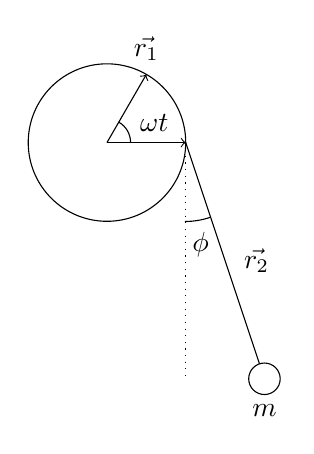
\begin{tikzpicture}
  \draw (0, 0) circle (1cm);
  \draw (1, 0) -- (2, -3);
  \draw [dotted] (1, 0) -- (1, -3);
  \draw (1.316, -0.948) arc (-71:-90:1);
  \node at (1.19, -1.3) {$\phi$};
  \node at (1.9, -1.5) {$\vec{r_2}$};
  \draw [fill=white] (2, -3) circle (0.2cm);
  \node at (2, -3.4) {$m$};
  \draw [->] (0, 0) -- (1, 0);
  \draw [->] (0, 0) -- (0.5, 1.73/2);
  \draw (0.3, 0) arc (0:60:0.3);
  \node at (0.5, 1.19) {$\vec{r_1}$};
  \node at (0.6, 0.25) {$\omega t$};

\end{tikzpicture}
\end{center}

Where, $\|\vec{r_1} \Vert = R$, $\|\vec{r_2} \Vert = L$; $m$ is the mass of the bob, $\phi$ is the angle of the pendulum, and $\omega t$ is how much the wheel rotates by in time t.
Adding $\vec{r_1}$ and $\vec{r_2}$:

$\vec{r_1}$ = 
$\begin{pmatrix}
  R \cos(\omega t) \\
  R \sin(\omega t)  
\end{pmatrix}$

\

$\vec{r_2}$ = 
$\begin{pmatrix}
  L \sin(\phi) \\
  -L \cos(\phi)  
\end{pmatrix}$

\

$\vec{r}$ = $\vec{r_1}$ + $\vec{r_2}$ = 
$\begin{pmatrix}
  R \cos(\omega t) + L \sin(\phi) \\
  R \sin(\omega t) - L \cos(\phi)  
\end{pmatrix}$

and so, \

$\vec{v}$ = $\cfrac{\mathrm{d} \vec{r}}{\mathrm{d} t}$ = 
$\begin{pmatrix}
  -R \omega \sin(\omega t) + L \dot{\phi} \cos(\phi) \\
  R \omega \cos(\omega t) + L \dot{\phi} \sin(\phi)  
\end{pmatrix}$

$T$ = $\frac{1}{2}mv^2$ = $\frac{1}{2} m (\vec{v} \cdot \vec{v})$
\\ \\
$\vec{v} \cdot \vec{v}$ :
\\ \\
$R^2 \omega^2 \sin^2(\omega t) + L^2 \dot{\phi}^2 \cos^2(\phi) - 2 R \omega L \dot{\phi} sin(\omega t) \cos(\phi) + R^2 \omega^2 \cos^2(\omega t) + L^2 \dot{\phi}^2 \sin^2(\phi) + 2 R \omega L \dot{\phi} cos(\omega t) \sin(\phi)$
\\ \\
= $R^2 \omega^2 (\sin^2(\omega t)+\cos^2(\omega t)) + L^2 \dot{\phi}^2 (\cos^2(\phi)+\sin^2(\phi)) + 2 R \omega L \dot{\phi}(cos(\omega t) \sin(\phi) - sin(\omega t) \cos(\phi))$
\\ 
= $R^2 \omega^2 + L^2 \dot{\phi}^2 + 2 R \omega L \dot{\phi}(\sin(\phi - \omega t))$
\\ \\
$T = \cfrac{m}{2} (R^2 \omega^2 + L^2 \dot{\phi}^2 + 2 R \omega L \dot{\phi}\sin(\phi - \omega t))$

and,

$U = mg{r_y} = mg(R \sin(\omega t) - L \cos(\phi))$
\\ \\
The Lagrangian, $\Lagr$ is defined as:
\begin{center}
  $\Lagr \equiv  T - U$
\end{center}
On substituting $T$ and $U$:
\\ \\
$\Lagr = \cfrac{m}{2} (R^2 \omega^2 + L^2 \dot{\phi}^2 + 2 R \omega L \dot{\phi}\sin(\phi - \omega t)) - mg(R \sin(\omega t) - L \cos(\phi))$ :

$\implies \cfrac{\partial \Lagr}{\partial \phi} = m R \omega L \dot{\phi} \cos(\phi - \omega t) - m g L \sin(\phi)$;
\\ \\
$\implies \cfrac{\partial \Lagr}{\partial \dot{\phi}} = m L^2 \dot{\phi} + m R \omega L \sin(\phi - \omega t)$,
\\ \\
$\implies \cfrac{d}{dt} \left( \cfrac{\partial \Lagr}{\partial \dot{\phi}} \right) = m L^2 \dot{\phi} + m R \omega L \sin(\phi - \omega t)$;
\\ \\ 
Plugging $\cfrac{\partial \Lagr}{\partial \phi}$ and $\cfrac{d}{dt} \left( \cfrac{\partial \Lagr}{\partial \dot{\phi}} \right)$ into the Euler-Lagrange equation, $\cfrac{\partial \Lagr}{\partial \phi} - \cfrac{d}{dt} \left( \cfrac{\partial \Lagr}{\partial \dot{\phi}} \right) = 0$, we get:
\\ \\
$m R \omega L \dot{\phi} \cos(\phi - \omega t) - m g L \sin(\phi) = m L^2 \ddot{\phi} + m R \omega L \dot{\phi} \cos(\phi - \omega t) - m R \omega^2 L \cos(\phi - \omega t)$
\\ \\
$\implies - m g L \sin(\phi) = m L^2 \ddot{\phi} - m R \omega^2 L \cos(\phi - \omega t)$
\\ \\
$\implies - g \sin(\phi) = L \ddot{\phi} - R \omega^2 \cos(\phi - \omega t)$

\begin{empheq}[box={\mybluebox[5pt][5pt]}]{equation*}
  L \ddot{\phi} + g \sin(\phi) = R \omega^2 \cos(\phi - \omega t)
\end{empheq}

This makes sense since for $\omega$ = 0 we have:
\\ \\
$L \ddot{\phi} + g \sin(\phi) = 0$
\\ \\
$\implies \ddot{\phi} = -\cfrac{g}{L} \sin(\phi)$
\\ \\
which is the differential equation for a pendulum (still VERY hard to solve). When $\omega = 0$, the wheel doesn't rotate, so all we have is a swinging pendulum. For small angles (small $\phi$) this DE reduces to the familiar $\ddot{\phi} = -\frac{g}{L} \phi$ which gives SHM.
\\ \\
\\ \\
\\ \\
\\ \\
(b)
\\ \\
Python code:
\begin{lstlisting}
  for omga in [0, 0.2]:
    def diffeqs(w, t, p):
        [phi, phid] = w # d matrix
        [L, g, R, omga] = p # parameters
        der =   [phid, 
                (R*omga*omga*mat.cos(phi - omga*t) - g*mat.sin(phi))/L]
        return der

    # initial conditions
    phi = 0.2
    phid = 0

    # time scale
    t = np.linspace(0, 20, 1000)

    # containing parameters and initial conditions
    p = [L, g, R, omga]
    w0 = [0.2, 0]

    wsol = odeint(diffeqs, w0, t, args = (p, ))
    #print(wsol[:, 0]) #prints the solution for corresponding x-range.
\end{lstlisting}

\begin{center}
  \makebox[0pt]{\includegraphics[scale=0.3]{20s.png}}
\end{center}

\begin{center}
  \begin{changemargin}{1cm}{1cm}  
Figure 1.1: We see that for $\omega = 0.2$ the amplitude of the pendulum decreases.
  \end{changemargin}
\end{center}

Since the DE, $L \ddot{\phi} + g \sin(\phi) = R \omega^2 \cos(\phi - \omega t)$ cannot be solved analytically, we use a computer to solve it. I used Python to plot the solution $\phi(t)$ from $t$ = 0 to $t$ = 20, as shown in Figure 1.1.
\\ \\
We solve the following DE using Python:
\begin{center}
  $\dfrac{d}{dt}$
$\begin{bmatrix}
  \phi \\
  \dot{\phi} 
\end{bmatrix}$
$ = $
$\begin{bmatrix}
  \dot{\phi}  \\
  \cfrac{R \omega^2 \cos(\phi - \omega t) - g \sin(\phi)}{L}
\end{bmatrix}$
\end{center} 
Where $R$, $L$, $g$, and $\omega$ are given parameters. Here, $R = 0.2$, $L = 1$, $g = 1$, and $\omega = 0, 0.2$.
\\ \\
For the first 20 seconds, we see that the amplitude decreases (overall). This makes more sense if we think about how the wheel moving towards the left causes the pendulum to ``not move to the left as much". Hence the upward shift seen in the first 5 seconds. It continues to swing like this for the next 5 seconds, since the wheel is still moving towards the left ($\approx$110°)
\\ \\
(c)
\begin{center}
  \makebox[0pt]{\includegraphics[scale=0.3]{120s.png}}
\end{center}

%\begin{center}
\begin{changemargin}{1cm}{1cm}  
  Figure 1.2: We see that for $\omega = 0.2$ and $t = 120s$ the envelope of $\phi$ changes.
\end{changemargin}
%\end{center}
For 120 seconds we see the bigger picture, the amplitude decreases and the envelope changes from two parallel straight lines to parallel cosine functions (approximately). The envelope has the same period as that of the wheel; the angle decreases to a minimum when the it is at $(0, -R)$, where the shift happens, i.e., where the wheel goes from "moving to the left" to "moving to the right"; and this, of course, happens all over again.
\\ \\
\\ \\
\\ \\
\item Diagram:

\begin{center}
  \begin{tikzpicture}
    \draw [dotted] (1, 2) -- (1, -3);
    \draw [dotted] (-1, 2) -- (-1, -3);
    \draw [fill = white] (0, 0) rectangle (2, 1);
    \draw (0.5, -0.2) circle (0.2cm);
    \draw (1.5, -0.2) circle (0.2cm); 
    \draw [->] (-1, 2) -- (1, 2);
    \draw [<-] (1.316, -0.948) arc (-71:-90:1);
    \node at (1.19, -1.3) {$\phi$};
    \node at (1.9, -1.5) {$\vec{r_2}$};
    \draw (1, 0) -- (2, -3);
    \draw [fill=white] (2, -3) circle (0.2cm);
    \draw [decoration={aspect=0.3, segment length=3mm, amplitude=3mm,coil},decorate] (-4, 0.5) -- (-1, 0.5);
    \draw (-1, 0.5) -- (0, 0.5);
    \draw (-5, 0.5) -- (-4, 0.5);
    \draw (-5, -0.4) -- (3, -0.4); 
    \draw (-5, -0.4) -- (-5, 3); 
    \node at (-2.65, 1.2) {$k$};
    \node at (1, 0.5) {$m$};
    \node at (1.95, -3.5) {$M$};
    \node at (0, 2.3) {$\vec{r_1}$};
    \draw [->] (-7, -0.4) -- (-6, -0.4);
    \draw [->] (-7, -0.4) -- (-7, -1.4);
    \node at (-5.8, -0.4) {$x$};
    \node at (-7, -1.65) {$y$};
  \end{tikzpicture}
  \end{center}

Where, $\|\vec{r_1} \Vert = x$, $\|\vec{r_2} \Vert = L$; $M$ is the mass of the bob, $m$ is the mass of the cart, $\phi$ is the angle of the pendulum, and $k$ is the spring constant.
Adding $\vec{r_1}$ and $\vec{r_2}$:
\\ \\
$\vec{r}_1$ = $\vec{r}_m$
 = $\begin{pmatrix}
  x \\
  0  
\end{pmatrix}$

\

$\vec{r}_2$ = 
$\begin{pmatrix}
  L \sin(\phi) \\
  -L \cos(\phi)  
\end{pmatrix}$

\

$\vec{r}_1$ + $\vec{r}_2$ = $\vec{r}_M$ = 
$\begin{pmatrix}
  x + L \sin(\phi) \\
  L \cos(\phi)  
\end{pmatrix}$

and so, \

$\vec{v}_m$ = $\cfrac{\mathrm{d} \vec{r}_m}{\mathrm{d} t}$ = 
$\begin{pmatrix}
  \dot{x} \\
  0  
\end{pmatrix}$

$T_m$ = $\frac{1}{2}mv_m^2$ = $\frac{1}{2} m (\vec{v}_m \cdot \vec{v}_m)$ = $\frac{1}{2} m \dot{x}^2$
\\ \\
$\vec{v}_M$ = $\cfrac{\mathrm{d} \vec{r}_M}{\mathrm{d} t}$ = 
$\begin{pmatrix}
  \dot{x} + L\dot{\phi}\cos{\phi}\\
  -L\dot{\phi}\sin(\phi)  
\end{pmatrix}$

$T_M = \frac{1}{2}mv_M^2$ = $\frac{1}{2} M (\vec{v}_M \cdot \vec{v}_M)$ = $\frac{1}{2} M (\dot{x}^2 + L^2 \dot{\phi}^2 \cos^2{\phi} + L^2 \dot{\phi}^2 \sin^2{\phi} + 2\dot{x}L\dot{\phi}\cos(\phi))$
\\ \\
$T_M = \frac{1}{2} M \dot{x}^2 + \frac{1}{2} M L^2 \dot{\phi}^2 + M \dot{x}L\dot{\phi}\cos(\phi))$
\\ \\
$T = T_m + T_M = \frac{1}{2} m \dot{x}^2 + \frac{1}{2} M \dot{x}^2 + \frac{1}{2} M L^2 \dot{\phi}^2 + M \dot{x}L\dot{\phi}\cos(\phi))$
\\ \\
\\ \\
$U_m = \frac{1}{2}kx^2$ (Potential energy of a spring)
\\ \\
$U_M = -mgr_M = -MgL\cos(\phi)$
\\ \\
$U = U_m + U_M = \frac{1}{2}kx^2 -MgL\cos(\phi)$
\\ \\
The Lagrangian, $\Lagr$ is defined as:
\begin{center}
  $\Lagr \equiv  T - U$
\end{center}
On substituting $T$ and $U$:
\\ \\
$\Lagr = \frac{1}{2} m \dot{x}^2 + \frac{1}{2} M \dot{x}^2 + \frac{1}{2} M L^2 \dot{\phi}^2 + M \dot{x}L\dot{\phi}\cos(\phi)) - \frac{1}{2}kx^2 +MgL\cos(\phi)$:
\\ \\
Since $\Lagr = \Lagr [ x(t), \phi (t), \dot{x}(t), \dot{\phi}(t), t]$, we have two Euler-Lagrange equations:
\\ \\
$\implies \cfrac{\partial \Lagr}{\partial x} = -kx$;
\\ \\
$\implies \cfrac{\partial \Lagr}{\partial \dot{x}} = (m+M)\dot{x} + ML\dot{\phi}\cos(\phi)$,
\\ \\
$\implies \cfrac{d}{dt} \left( \cfrac{\partial \Lagr}{\partial \dot{x}} \right) = (m+M)\ddot{x} + ML(\cos(\phi)\ddot{\phi} - \sin(\phi)\dot{\phi}^2)$;
\\ \\ 
Plugging $\cfrac{\partial \Lagr}{\partial x}$ and $\cfrac{d}{dt} \left( \cfrac{\partial \Lagr}{\partial \dot{x}} \right)$ into the Euler-Lagrange equation, $\cfrac{\partial \Lagr}{\partial x} - \cfrac{d}{dt} \left( \cfrac{\partial \Lagr}{\partial \dot{x}} \right) = 0$, we get:
\\ \\
$-kx = (m+M)\ddot{x} + ML(\cos(\phi)\ddot{\phi} - \sin(\phi)\dot{\phi}^2)$
\\ \\
$\implies (m+M)\ddot{x} + ML(\cos(\phi)\ddot{\phi} - \sin(\phi)\dot{\phi}^2) + kx = 0$

\begin{empheq}[box={\mybluebox[5pt][5pt]}]{equation*}
  (m+M)\ddot{x} + ML(\cos(\phi)\ddot{\phi} - \sin(\phi)\dot{\phi}^2) + kx = 0 \ \ \ \ (2.1)
\end{empheq}

$\implies \cfrac{\partial \Lagr}{\partial \phi} = -ML\dot{\phi}\dot{x}\sin(\phi) - MgL\sin(\phi)$;
\\ \\
$\implies \cfrac{\partial \Lagr}{\partial \dot{\phi}} =  ML^2\ddot{\phi} + ML\ddot{x}\cos(\phi) - ML\dot{x}\dot{\phi}\sin(\phi))$,
\\ \\
$\implies \cfrac{d}{dt} \left( \cfrac{\partial \Lagr}{\partial \dot{\phi}} \right) = ML^2\ddot{\phi} + ML\ddot{x}\cos(\phi) - ML\dot{x}\dot{\phi}\sin(\phi)$;
\\ \\
Plugging $\cfrac{\partial \Lagr}{\partial \phi}$ and $\cfrac{d}{dt} \left( \cfrac{\partial \Lagr}{\partial \dot{\phi}} \right)$ into the Euler-Lagrange equation, $\cfrac{\partial \Lagr}{\partial \phi} - \cfrac{d}{dt} \left( \cfrac{\partial \Lagr}{\partial \dot{\phi}} \right) = 0$, we get:
\\ \\
$g\sin(\phi) + L\ddot{\phi} + \ddot{x}\cos(\phi) = 0$
$\implies M(L\ddot{\phi} + \cos(\phi)\ddot{x}) + Mg\sin(\phi) = 0$
\begin{empheq}[box={\mybluebox[5pt][5pt]}]{equation*}
%\begin{equation}
  M(L\ddot{\phi} + \cos(\phi)\ddot{x}) + Mg\sin(\phi) = 0 \ \ \ \ (2.2)
%\end{equation}
\end{empheq} 


(b)
\\ \\
Python code:
\begin{lstlisting}
  #parameters
  m = 1
  M = 1
  L = 1
  g = 1
  k = 2

  def diffeqs(w, t, p):
      [x, phi, xd, phid] = w # d matrix
      [m, M, L, g, k] = p # parameters
      der =   [xd, 
              phid, 
              (M*L*phid*mat.sin(phi) - k*x + M*g*mat.sin(phi)*mat.cos(phi))/((m+M) - M*(mat.cos(phi)*mat.cos(phi))),
              (M*M*mat.cos(phi)*mat.sin(phi)*L*phid*phid - M*mat.cos(phi)*k*x + (M+m)*M*g*mat.sin(phi))/((M*M*L*mat.cos(phi)*mat.cos(phi)) - ((M+m)*M*L))]
      return der

  # initial conditions
  #x = 0
  #phi = 0
  #xd = 0 
  #phid = 0

  # time scale
  t = np.linspace(0, 3, 10000)

  # containing parameters and initial conditions
  p = [m, M, L, g, k]
  w0 = [0.1, 0, 0, 0]


  wsol = odeint(diffeqs, w0, t, args = (p, ))
\end{lstlisting}

Note that we get expressions for $\ddot{\phi}$ and $\ddot{x}$ from the two Euler-Lagrange equations, i.e. equations 2.1 and 2.2. So, using Python, we solve (YIKES!):
\begin{center}
  $\dfrac{d}{dt}$
$\begin{bmatrix}
  x \\
  \phi \\
  \dot{x} \\
  \dot{\phi} 
\end{bmatrix}$
$ = $
$\begin{bmatrix}
  \dot{x} \\
  \dot{\phi} \\
  \cfrac{ML\dot{\phi}\sin(\phi) - kx + Mg\sin(\phi)\cos(\phi)}{(m+M) - M\cos^2(\phi)} \\
  \cfrac{M^2L\dot{\phi}^2\cos(\phi)\sin(\phi) - Mkx\cos(\phi) + (m+M)Mg\sin(\phi)}{M^2 L \cos^2(\phi) - (m+M)ML}
\end{bmatrix}$
\end{center}

Where $m = 1, M = 1, L = 1, g = 1,$ and $k = 2$ are the given parameters.

\begin{center}
  \makebox[0pt]{\includegraphics[scale=0.25]{3s.png}}
\end{center}

\begin{changemargin}{3cm}{3cm}  
  Figure 2.1: After solving the differential equation, we get the above plot for $x(t)$ and $\phi(t)$.
\end{changemargin}

The plot is just as we would expect, intitially since the spring is extended by $x = 0.1$ from equilibrium, it begins to move ``backwards" causing $x$ to decrease. Meanwhile, the pendulum that is in its equilibrium postion with no angular velocity (as according to given initial conditions), ``stays" or ``tends to stay" behind because of inertia. This causes $\phi$ to increase since the pendulum is constrained. After $x$ drops to a minimum (not $-x$ because of the pendulum), the pendulum continues to swing causing $\phi$ to decrease before the cart $x$ increases again, which is why there is a delay at $t = 2s$, i.e. the waves are not in sync.
\\ \\
(c)
\begin{center}
  \makebox[0pt]{\includegraphics[scale=0.25]{30s.png}}
\end{center}

\begin{changemargin}{3cm}{3cm}  
  Figure 2.2: For $\phi(0) = x(0)\sqrt{2}$ we see that the two plots are ``in sync".
\end{changemargin}

When we change $\phi(0)$ to $x(0)\sqrt{2}$ (here, $0.1\sqrt{2}$) we get the plot in Figure 2.2. As the pendulum goes from tis initial $\phi = sqrt{2}x(0)$ to $\phi = -sqrt{2}x(0)$, the cart goes from its initial $x = 0.1$ to $x = -0.1$. On zooming into the graph using Python's interactive graph output, we see that the period of both the crate and the pendulum is $\approx 8.38s$.
\\ \\
\\ \\
\\ \\
\\ \\
Bonus plot:

\begin{center}
  \makebox[0pt]{\includegraphics[scale=0.3]{bonus_0.png}}
\end{center}

\begin{changemargin}{3cm}{3cm}  
  Figure 3.1: Shows the evolution of the system from question 1 for $\omega$ going from 0 to 2 in steps of 0.1.
\end{changemargin}

\end{enumerate}

\end{document}